\documentclass[12pt,parskip=full,ngerman]{scrartcl}
\usepackage{graphicx}
\usepackage{tikz}
\usepackage[placement=top]{background}
\usepackage{xcolor}
\usepackage[a4paper,left=20mm,right=10mm,top=25mm,bottom=10mm,includeheadfoot]{geometry}
\usepackage[ngerman]{babel}
\usepackage{tabularx}
\usepackage{blindtext}
\usepackage{paracol}
\usepackage{lipsum}
\usepackage{csquotes}
\usepackage{enumitem}
\usepackage{makecell}
\usepackage{lastpage}
\usepackage{fancyhdr}
\usepackage{amsmath,amssymb}
\usepackage{eforms}
\usepackage{pdfpages}
\usepackage{ifthen}
\usepackage{ifluatex}
%\ifluatex
%	\usepackage{unicode-math}
%	\setmainfont{Latin Modern Roman}
%	\setsansfont{Latin Modern Sans}
%	\setmonofont{Latin Modern Mono}
%	\setmathfont{Latin Modern Math}
%\else % pdflatex
	\usepackage[utf8]{inputenc}
	\usepackage[T1]{fontenc}
	\usepackage{lmodern}
%\fi

% first add the transparent lily to the background
% angle and position are taken from the DPSG style guide. Exact size may not be perfect, but good enough
% opacity should be 30% as per the style guide, but that is a little to dark (their examples also look lighter)
\backgroundsetup{contents=
\includegraphics{pictures/lilie_outline}, scale=0.35, opacity=0.27, angle=5, position={-3mm, 38mm}}
\makeatletter

% add the end page marker in the bottom right to the background
\AddEverypageHook{% 
	\SetBgContents{\tikz [remember picture, overlay]
		\node [shift={(-11mm, 7mm)}] at (current page.south east) %
		[anchor=south east] %
		{
\includegraphics{pictures/end}};
	}
	\SetBgPosition{current page.south east}
	\SetBgHshift{0}
	\SetBgVshift{0}  
	\SetBgOpacity{1}
	\SetBgAngle{0}
	\SetBgScale{1}
	\bg@material
}

% for formatting the entries in the sidebar
\NewDocumentCommand{\vorstand}{mmmO{}}{%
	\textbf{#1}\\
	#2\\
	#3\\
	\IfNoValueTF{#4}{}{#4\\}
	\vspace{5mm}
}

% styling options for the form fields
\everyTextField{\BG{beaublue}\BC{gray}\textSize{14}}
\everyRadioButton{\BG{beaublue}\BC{gray}\symbolchoice{check}}

% shorthands to make form code more readable
\newcommand{\br}{\\[16pt]}
\newcommand{\h}{1.5\baselineskip}

% set font
\renewcommand*\familydefault{\sfdefault}

\definecolor{beaublue}{rgb}{0.74, 0.83, 0.9} % form background
\definecolor{dpsgbeige}{RGB}{199,189,173}
\definecolor{dpsgblue}{RGB}{0,48,86}

% colour the section headings in dpsgblue and add the red start marker to each \section heading
\newsavebox\mybox
\newsavebox\imagebox
\addtokomafont{section}{%
	\sbox{\mybox}{\thesection}
	\sbox{\imagebox}{%
		
\includegraphics{pictures/start}
	}
	\hspace*{-\wd\mybox}
	\hspace*{-\wd\imagebox}
	
\includegraphics[trim=0.7cm -0.5mm 0 0]{pictures/start}
	\hspace{0.5em}
	\color{dpsgblue}
}
\addtokomafont{subsection}{%
	\color{dpsgblue}
}
\addtokomafont{subsubsection}{%
	\color{dpsgblue}
}
\addtokomafont{paragraph}{%
	\color{dpsgblue}
}
\addtokomafont{title}{%
	\color{dpsgblue}
}

% add the pagenumber to the bottom left
\hypersetup{
	colorlinks=true, % Set this to false if you prefer default colored boxes around form fields
	linkcolor=black,
}
\fancyfoot[L]{\small Page \thepage\ of \pageref{LastPage}}
\cfoot{}
\renewcommand{\headrulewidth}{0pt} 

% used by pandoc
\providecommand{\tightlist}{%
  \setlength{\itemsep}{0pt}\setlength{\parskip}{0pt}}


% add generated settings from API input
\newboolean{includeSignUp}
\setboolean{includeSignUp}{true}
\newboolean{includeFrontPage}
\setboolean{includeFrontPage}{true}
\newboolean{includeHolidayLawPage}
\setboolean{includeHolidayLawPage}{true}
\newboolean{signUpIncludeAbroadClause}
\setboolean{signUpIncludeAbroadClause}{true}
\newcommand{\currentDate}{19.10.2024}
\newcommand{\place}{string}
\newcommand{\address}{string}
\newcommand{\orgName}{string}
\newcommand{\personOneName}{string}
\newcommand{\personOneRole}{Stammesvorsitzender}
\newcommand{\personOneEmail}{string}
\newcommand{\personTwoName}{string}
\newcommand{\personTwoRole}{Stammesvorsitzender}
\newcommand{\personTwoEmail}{string}
\newcommand{\bankOrgName}{string}
\newcommand{\bankName}{string}
\newcommand{\iban}{string}
\newcommand{\logoFile}{pictures/logos/langenbach_logo_cropped}
\newcommand{\logoWidth}{4.6cm}
\newcommand{\logoShiftX}{-0.5cm}
\newcommand{\logoShiftY}{-0.5cm}


\begin{document}
	
\ifthenelse{\boolean{includeFrontPage}}{
	
\thispagestyle{empty}

% shift values taken from DPSG style guide, might not work perfectly for other logos
\tikz [remember picture, overlay] %
\node [shift={(\logoShiftX,\logoShiftY)}] at (current page.north east) %
%\node [shift={(-0.6cm,-1.3cm)}] at (current page.north east) %
[anchor=north east] %
{\includegraphics[width=\logoWidth]{\logoFile}};


\columnratio{0.73,0.02,0.25}
\begin{paracol}{3}
	\raggedright
	\begin{nthcolumn}{0}
		\section*{string}

string

	\end{nthcolumn}
	\begin{nthcolumn}{2}
		\footnotesize
\vspace{10mm}
%
\place, \currentDate\\
%
\vspace{10mm}
\scriptsize
\textbf{Kontakt}\\
%
\orgName\\
\address\\
%
\ifdefined\website
    \vspace{\heightof{X}}
    \website\\
\fi
\vspace{5mm}
%
%
\@ifundefined{personOnePhone}{
    \vorstand{\personOneName}{\personOneRole}{\personOneEmail}
}{
    % TODO maybe format + in phone number differently
    \vorstand{\personOneName}{\personOneRole}{\personOneEmail}[\personOnePhone]
}
\@ifundefined{personTwoPhone}{
    \vorstand{\personTwoName}{\personTwoRole}{\personTwoEmail}
}{
    \vorstand{\personTwoName}{\personTwoRole}{\personTwoEmail}[\personTwoPhone]
}
% only add third person if it is defined
\ifdefined\personThreeName
    \@ifundefined{personThreePhone}{
        \vorstand{\personThreeName}{\personThreeRole}{\personThreeEmail}
    }{
        \vorstand{\personThreeName}{\personThreeRole}{\personThreeEmail}[\personThreePhone]
    }
\fi

%
\vspace{10mm}
\textbf{Kontoverbindung}\\
\bankOrgName\\
\bankName\\
IBAN:\\
\iban
	\end{nthcolumn}
\end{paracol}
\newpage
}{}%endif

\ifthenelse{\boolean{includeHolidayLawPage}}{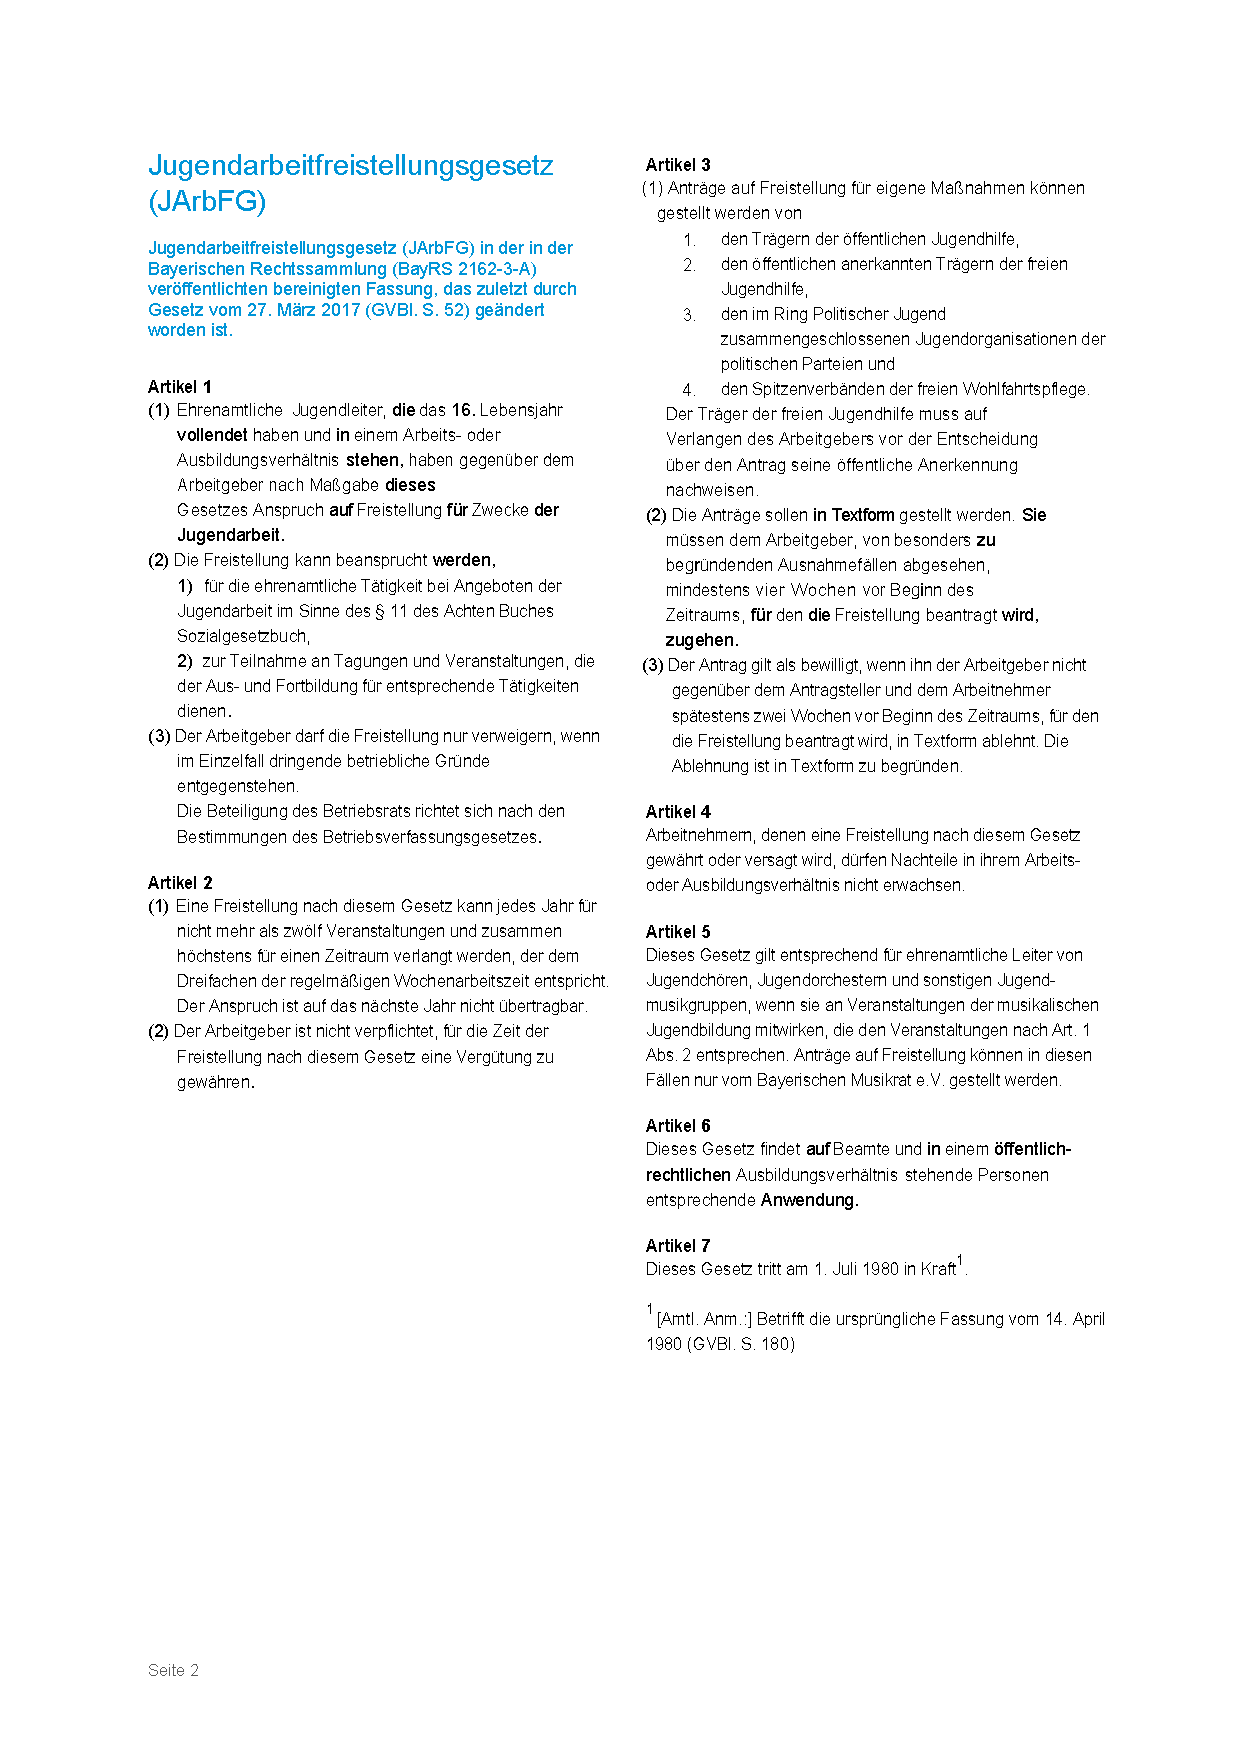
\includepdf[pagecommand={\thispagestyle{empty}}]{content/jugendarbeitsfreistellungsgesetz.pdf}}{}

\ifthenelse{\boolean{includeSignUp}}{
% reset margins to reduce wasted space at the top of the page
\newgeometry{a4paper,left=20mm,right=15mm,top=10mm,bottom=5mm,includeheadfoot}

\pagestyle{fancy}
\setcounter{page}{1}

% for multicolumn in the "Lebensmittelunverträglichkeiten" row
\newlength{\yhwidth}
\newcommand{\yhmulticolumn}[4]{\multicolumn{#2}{#3}{\settowidth{\yhwidth}{#1}\hsize=\dimexpr\hsize+\yhwidth+2\tabcolsep+\arrayrulewidth\relax #4}}

\section*{Anmeldung}
\small
\begin{Form}
    %\newcommand{\arraystretch}{1.3}%
    \begin{tabularx}{\linewidth}{lX}
        Für die Aktion: & \textField{aktion}{\linewidth}{\h} \br
        Zeitraum: & \textField{zeitraum}{\linewidth}{\h}
    \end{tabularx}

    \subsection*{Teilnehmer*in}
    \begin{tabularx}{\linewidth}{lX}
        *Name: & \textField{name}{\linewidth}{\h}\br
        *Vorname: & \textField{surname}{\linewidth}{\h}\br
        *Geburtsdatum: & \textField{birthdate}{\linewidth}{\h}\br
        *Gruppe: & \textField{gruppe}{\linewidth}{\h}\br
        *Gruppenleiter*in: & \textField{leitung}{\linewidth}{\h}\br
        *Anschrift: & \textField{address}{\linewidth}{\h}
    \end{tabularx}

    \begin{tabularx}{\linewidth}{lll}
        *Mein Kind ist:
        & \mbox{\radioButton{swim}{15bp}{15bp}{}\quad Schwimmer*in\quad}
        & \mbox{\radioButton{swim}{15bp}{15bp}{}\quad Nichtschwimmer*in}\br

        *Ernährung:
        & \mbox{\radioButton{essen}{15bp}{15bp}{}\quad Vegan\qquad}
        & \mbox{\radioButton{essen}{15bp}{15bp}{}\quad Vegetarisch\qquad}
        \mbox{\radioButton{essen}{15bp}{15bp}{}\quad Alles}\br

        *Lebensmittelunverträglichkeit: & \yhmulticolumn{}{2}{X}{\textField{lebensmittel}{\linewidth}{\h}}
    \end{tabularx}

    \subsection*{Eltern}
    \begin{tabularx}{\linewidth}{lX}
        *Namen der Eltern: & \textField{eltern}{\linewidth}{\h}\br
        *Anschrift d.E.\ während der Aktion: & \textField{addressParents}{\linewidth}{\h}\br
        *Telefonnummer d.E.\ während der Aktion: & \textField{phone}{\linewidth}{\h}
    \end{tabularx}

    \subsection*{Versicherung / Medizinische Versorgung}
    \begin{tabularx}{\linewidth}{lX}
        *Krankenkasse:
        & \mbox{\radioButton{kk}{15bp}{15bp}{}\quad Gesetzlich}\quad\mbox{\radioButton{kk}{15bp}{15bp}{}\quad Privat}\br

        *Nummer der KK: & \textField{kkNumber}{\linewidth}{\h}\br
        *Name der KK: & \textField{kkName}{\linewidth}{\h}\br
        *Hausärzt*in: & \textField{doctor}{\linewidth}{\h}\br
        *Impfung gegen FSME bis: & \textField{fsme}{\linewidth}{\h}\br
        *Impfung gegen Tetanus am: & \textField{tetanus}{\linewidth}{\h}\br
        Allergien / Krankheiten: & \textField{allergies}{\linewidth}{\h}\br
        \makecell[l]{
            Mein Kind muss folgende\\Medikamente regelmäßig einnehmen:
        }& \textField{medikament}{\linewidth}{\h}
    \end{tabularx}

    \ifthenelse{\boolean{signUpIncludeAbroadClause}}{
        \subsection*{Bei Fahrten ins Ausland}
        \begin{tabularx}{\linewidth}{lX}
            Personalausweis/Reisepass-nummer: & \textField{idNumber}{\linewidth}{\h}\\
            Mein Kind hat die Erlaubnis zum Grenzübertritt.
        \end{tabularx}
    }{}%endif

    \subsection*{Einverständniserklärung}
    Hiermit melde ich mich / mein Kind verbindlich zur Teilnahme an der oben genannten Aktion an.\\
    Wir erlauben in dringenden Fällen jeden unbedingt notwendigen ärztlichen Eingriff (z.B.\ Blinddarm).\\\\
    Ich stimme der \enquote{Vereinbarung über die Nutzung von Fotografien und Filmen} (Seite 3) zu:\br
    \hspace*{1cm}\mbox{\radioButton{kk}{15bp}{15bp}{}\quad Ja}\quad\mbox{\radioButton{kk}{15bp}{15bp}{}\quad Nein}\\

    \vspace*{1cm}
    \footnotesize
    \begin{tabularx}{\linewidth}{p{7cm}X}
        \noindent\hrulefill & \noindent\hrulefill                                            \\
        Ort, Datum          & Unterschrift Teilnehmer*in (\textbf{ab 13 Jahre erforderlich}) \\
        &                                                                \\
        &                                                                \\
        &                                                                \\
        \noindent\hrulefill & \noindent\hrulefill                                            \\
        Ort, Datum          & \makecell[l]{Unterschrift der Erziehungsberechtigten           \\\textbf{(Bei allen Minderjährigen unter 18 notwendig)}}
    \end{tabularx}
\end{Form}
\clearpage


\subsubsection*{VEREINBARUNG ÜBER DIE NUTZUNG VON FOTOGRAFIEN UND FILMEN FÜR BERICHTERSTATTUNG DER 
	DEUTSCHEN PFADFINDERSCHAFT SANKT GEORG (DPSG)/\MakeUppercase{\orgName} DER DEUTSCHEN
	PFADFINDERSCHAFT SANKT GEORG (DPSG)}
Zwischen dem Stamm \enquote{\orgName} der Deutschen Pfadfinderschaft Sankt Georg (DPSG) und o.g.\ Person wird folgende Nutzungsvereinbarung für Fotografien und
Videos getroffen:

\begin{enumerate}
	\item Es wird zugestimmt, dass von der o.g.\ Person Aufnahmen erstellt und der DPSG unentgeltlich zum
	Zwecke der Berichterstattung in Medien, zur Werbung und zur Verwendung nach Ziffer 2 zur 
	Verfügung gestellt werden.
	\item Für die Nutzung wird keine inhaltliche, zeitliche oder räumliche Beschränkung vereinbart.
	Der Nutzung für folgende Zwecke wird uneingeschränkt zugestimmt:
	\begin{itemize}[noitemsep]
		\item Veröffentlichung in den Medien des Stammes (z.B.\ Zeitschrift, Newsletter)
		\item Veröffentlichung in der Presse (z.B.\ Pressefotos)
		\item Veröffentlichung im Internet (z.B.\ auf den Homepages des Stammes oder den Auftritten des
		Stammes bei Facebook, YouTube, WhatsApp, Instagram etc.)
	\end{itemize}
	\item Die/der Fotografierte/Gefilmte stimmt einer Nutzung ihres/seines Fotos/Films zur Nutzung innerhalb 
	von Fotomontagen unter Entfernung oder Ergänzung von Bildbestandteilen bzw.\ für verfremdete
	Bilder der Originalaufnahmen zu.
	\item Ein Anspruch auf eine Nutzung im Sinne der Ziffern 1 und 2 wird durch diese Vereinbarung nicht 
	begründet.
	Der/die Fotografierte/Gefilmte kann bei \orgName über die
	Stammesvorstände die Art der Bild-Nutzung jederzeit erfragen.
	\item Die/der Fotografierte/Gefilmte überträgt dem Fotografen alle zur Ausübung der Nutzung gem.\ Ziffer 2
	notwendigen Rechte an den erstellten Fotografien und Filmen.
	\item Der Name der/des Fotografierten/ Gefilmten wird im Sinne des Datenschutzes nicht veröffentlicht. 
	Eine Weitergabe zum Zwecke der Markt- und Meinungsforschung findet nicht statt.
	\item Ein Honorar für die Fotografien und Filme wird vom DPSG Bundesverband nicht gezahlt.
	\item Eine Veränderung an dieser Vereinbarung bedarf der Schriftform.
\end{enumerate}

}{}%endif
\end{document}
